%!TEX root = Slic3r-Manual.tex

\section{Refroidissement} % (fold)
\label{sec:cooling}
\index{cooling}
\index{refroidissement}
\index{temperature}

La temp\'erature joue un r\^ole cl\'e dans la d\'etermination de la qualit\'e d'impression. Trop de chaleur produit des d\'eformation du mod\`ele, pas assez de chaleur pose des probl\`eme d'adh\'esion de la couche. L'application d'un refroidissement permettra au mat\'eriau fra\^ichement d\'epos\'e de se solidifier suffisament pour fournir une bonne base pour la couche suivante, aidant \`a la tenue des surplombs, des petits d\'etails et des ponts.

Il existe deux techniques principales pour le refroidissement: l'ajout d'un ventilateur, et ralentir la vitesse d'impression. Slic3r peut choisir d'utiliser les deux techniques, en utilisant d'abord un ventilateur, puis le ralentissement de l'impression si le temps de d\'epot de la couche est trop court.

\begin{figure}[H]
\centering
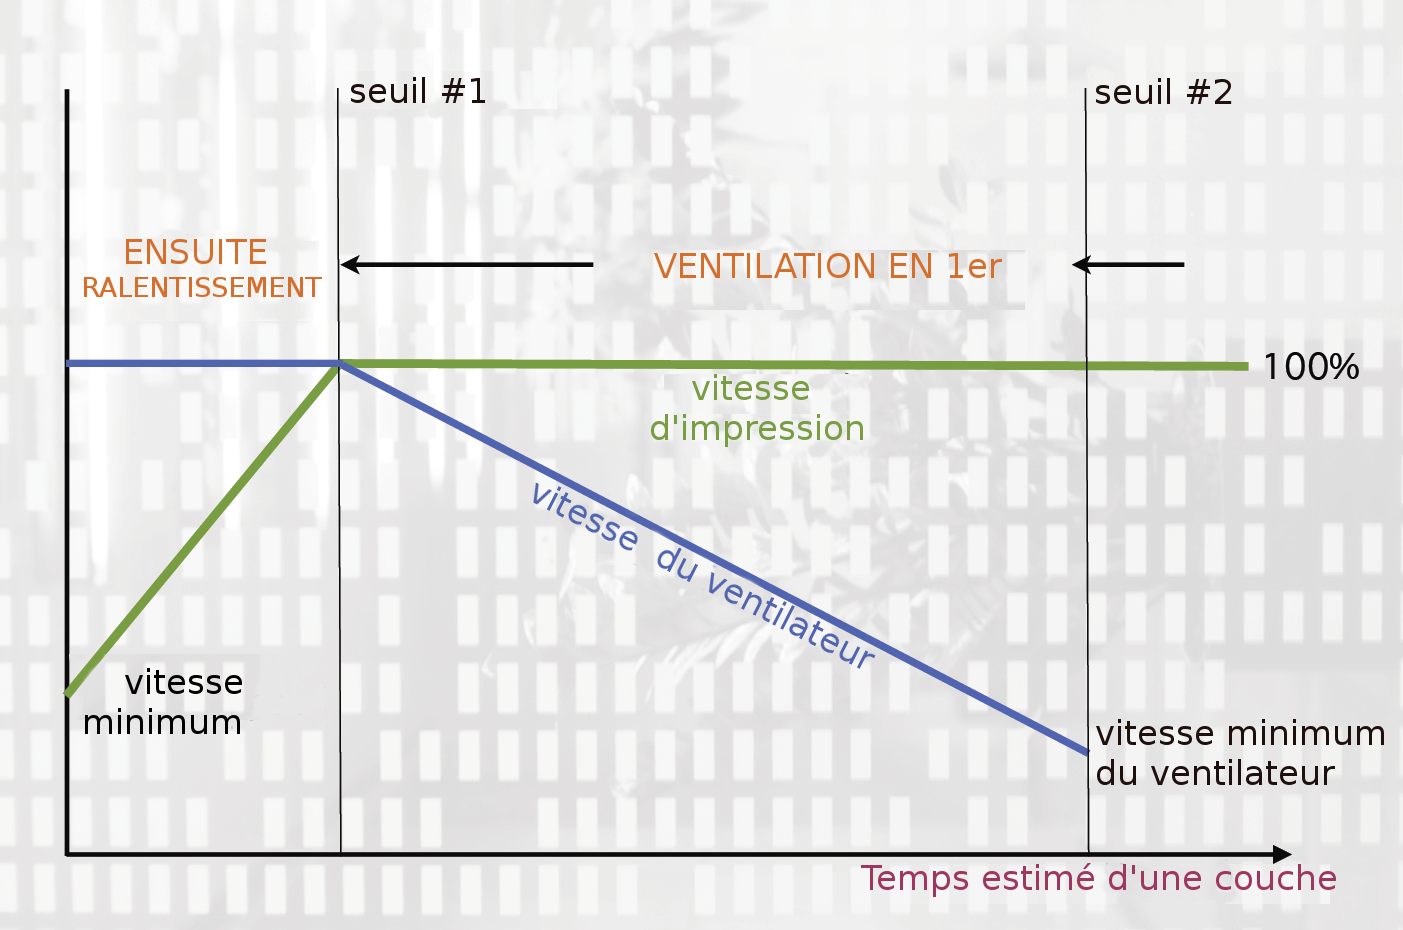
\includegraphics[keepaspectratio=true,width=1\textwidth]{expertmode/cooling_chart.png}
\caption{Strat\'egie de refroidissement.}
\label{fig:cooling_chart}
\end{figure}

La figure \ref{fig:cooling_chart} montre la strat\'egie adopt\'ee par Slic3r. La lecture se fait de droite \`a gauche, lorsque le seuil minimum du ventilateur (\#2) est atteint, le ventilateur, est activ\'e. Ceci augmente en intensit\'e \`a mesure que le temps de d\'epot de la couche diminue. La vitesse d'impression reste constante jusqu'\`a ce que le temps estim\'e d'impression descende au-dessous d'un certain seuil (\#1), c'est le moment o\`u la vitesse d'impression est r\'eduite jusqu'\`a ce qu'elle atteigne sa valeur minimale.

\subsection{Ventilateurs} % (fold)
\label{sub:fans}
\index{cooling!fans}
\index{refroidissement!ventilateurs}
La plupart des cartes \'electroniques et firmware permettent l'ajout de ventilateurs, via un connecteur disponnible. Ceux-ci peuvent ensuite \^etre pilot\'e avec le G-code, de Slic3r, pour activer ou d\'esactiver lorsque le mod\`ele le n\'ecessite, et de tourner \`a des vitesses diff\'erentes.

Des pr\'ecautions doivent \^etre prises avec le positionnement du ventilateur de sorte qu'il ne refroidisse pas de lit chauff\'e plus que n\'ecessaire. Il convient \'egalement de ne pas refroidir le bloc chauffant de la t\^ete afin de d\'eviter le gaspillage d'\'energie. Le mouvement de l'air devrait viser la pointe de la buse, o\`u coule sur le produit fra\^ichement extrud\'e.

Un conduit peut aider \`a guider le flux correctement, et il ya plusieurs mod\`eles disponibles en ligne, pour une grande vari\'et\'e d'imprimantes.

% subsection fans (end)

\subsection{Ralentissement} % (fold)
\label{sub:slowing_down}
\index{cooling!slowing down}
\index{refroidissement!ralentissement}
Slic3r peut indiquer \`a l'imprimante de ralentir si le temps de couche estim\'e est inf\'erieur \`a un certain seuil.

Attention, l'effet escompt\'e pourrait \^etre att\'enu\'e par le fait que la buse ne bouge pas assez loin de l'extrusion fra\^ichement d\'epos\'ee, c'est un probl\`eme avec les petits objets, les couches d\'etaill\'ees. Pour cette raison, il est g\'en\'eralement recommand\'e d'utiliser un ventilateur si possible.
% subsection slowing_down (end)

\subsection{Configuration} % (fold)
\label{sub:configuring_cooling}

En mode simple Slic3r tentera de choisir les param\`etres optimaux pour les ventilateur et la vitesse. Le mode expert donne plus d'options fines.

\begin{figure}[H]
\centering
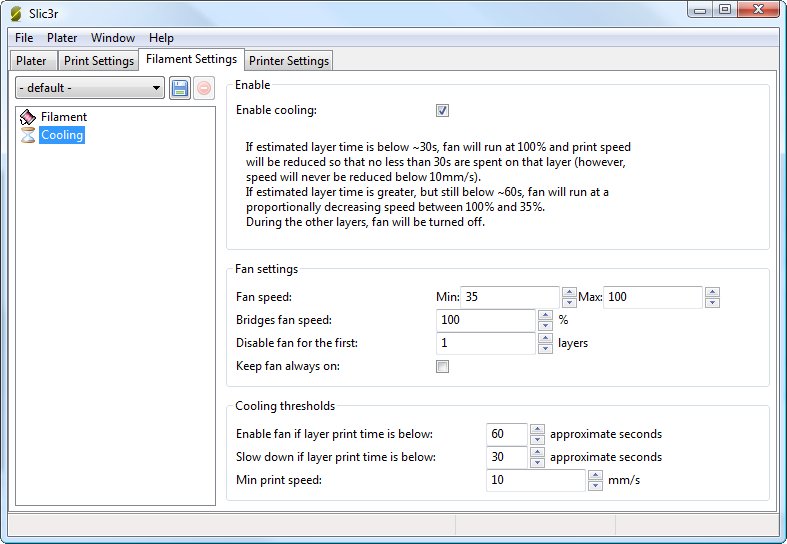
\includegraphics[keepaspectratio=true,width=1\textwidth]{expertmode/cooling_advanced_settings.png}
\caption{Param\`etres avanc\'es de refroidissement}
\label{fig:cooling_advanced_settings}
\end{figure}

\begin{itemize}
    \index{Filament Settings!Cooling!Fan speed}
	\index{Param\`etres du Filament!Refroidissement!Vitesse du ventilateur}
	\item \texttt{Fan speed} (Vitesse du ventilateur) - D\'etermine la vitesse minimum et maximum - utile pour les ventilateurs qui vont trop vite par d\'efaut.
    \index{Filament Settings!Cooling!Bridges fan speed}
	\index{Param\`etres du Filament!Refroidissement!Vitesse du ventilateur pour les ponts}
	\item \texttt{Bridges fan speed} (Vitesse du ventilateur pour les ponts) - Comme la mati\`ere s'\'etire dans le vide sur de grands \'ecarts, il est logique d'essayer de la refroidir autant que possible, donc la vitesse maxi du ventilateur est recommand\'e.
    \index{Filament Settings!Cooling!Disable fan for first n layers}
	\index{Param\`etres du Filament!Refroidissement!D\'esactiver le ventilateur pour les n 1ere couches}
	\item \texttt{Disable fan for first \textit{n} layers} (D\'esactiver le ventilateur pour les \textit{n} 1ere couches) - La section \ref{sec:the_important_first_layer} montre l'importance de la premi\`ere couche , il est donc logique de ne pas appliquer le ventilateur jusqu'\`a ce que l'impression soit solidement fix\'e au lit. Garder le ventilateur \'eteint pendant les deux ou trois premi\`eres couches est une bonne id\'ee.
    \index{Filament Settings!Cooling!Keep fan always on}
	\index{Param\`etres du Filament!Refroidissement!Garder le ventilateur allum\'e}
	\item \texttt{Keep fan always on} (Garder le ventilateur allum\'e) - Remplace tous les autres choix et force le ventilateur \`a fonctionner continuellement, au moins \`a la vitesse minimum. Cela peut \^etre utile lors de l'impression du PLA, mais n'est pas recommand\'e pour l'ABS ..
\end{itemize}

\begin{itemize}
    \index{Filament Settings!Cooling!Enable fan if print time is below t seconds}
	\index{Param\`etres du Filament!Refroidissement!Activer le ventilateur si temps d'impression inf\'erieur \`a t secondes}
	\item \texttt{Enable fan if print time is below \textit{t} seconds}  (Activer le ventilateur si temps d'impression inf\'erieur \`a \textit{t} secondes) - D\'eclenche le ventilateur, si la couche sera termin\'e dans le nombre donn\'e de secondes.
    \index{Filament Settings!Cooling!Slow down if layer print time is below t seconds}
	\index{Param\`etres du Filament!Refroidissement!Ralentir si temps d'impression inf\'erieur \`a t secondes}
	\item \texttt{Slow down if layer print time is below \textit{t} seconds}  (Ralentir si temps d'impression inf\'erieur \`a \textit{t} secondes) - Ralentit l'impression si la couche sera termin\'e dans le nombre donn\'e de secondes.
    \index{Filament Settings!Cooling!Min print speed}
	\index{Param\`etres du Filament!Refroidissement!Vitesse d'impression minimum}
	\item \texttt{Min print speed}  (Vitesse d'impression minimum) - Une limite inf\'erieure de la lenteur avec laquelle une couche peut \^etre imprim\'e.
\end{itemize}


% subsection configuring_cooling (end)

% section cooling (end)